
\section{Planning}

We will now discuss the idea of planning in RL. Planning is fundamental to the AlphaZero algorithm. Planning in the context of RL simply means any way in which an agent can use a model of the environment to improve upon a current policy. Either a global or local policy. We have mentioned models already but just to reiterate that a model is anything by which an agent can make predictions about what the environment will do next based on its own actions / interaction with that environment. This is actually intuitive as it is what a lot of us do well trying to make a decision in various domains. Think about trying to make a decision in your favorite game. You usually think along the lines "If I do this then they will do that and then if they do that I will do this...". You think about possible options and then what those various options could lead to. This usually leads to local improvements in your policy since you are just thinking about the current state and what is the best thing to do from there. There are various ways to do planning in RL but we will focus on what is called decision time planning. Decision time planning is what you do when thinking about making a decision in a game as we just discussed. The other way would be to plan from a more global perspective as we do with dynamic programming. That is before we select an action for any particular state we have done a whole lot of planning to compute a value function across all states. In the decision time planning perspective we are focused on a particular state and once we have decided on what action to take the planning process starts over again on the next state. We will see that this is what monte carlo tree search does and it the decision time planning algorithm used by AlphaZero.

Monte Carlo tree search is also a form of what is called a "rollout algorithm". Rollout algorithms are decision-time planning algorithms but they are based on Monte Carlo control which we discussed earlier. They use Monte Carlo control on simulated trajectories. Simulated trajectories are trajectories of state action pairs starting from a given state and go until a terminal state is reached. These state action pairs are sampled according to the current policy. So one simply samples an action from a starting state and then uses a model of the environment to get a next state then from that state the process is repeated until a terminal state is reached. This can be done until you have a number of trajectories sampled from a given state. Then you can simply average the returns for each of the actions from the current state to get an estimate of the state-action value for each one. 

Thinking back to the policy improvement theorem we know that if we can come up with a policy $\pi^{'}$ that is identical to the current policy except that for some action $q_{\pi}(s,a) \geq v_{\pi}(s)$ then we can say that $\pi^{'}$ is better than $\pi$. The sampled trajectories that we got from our rollout algorithm gives us an estimate of $q_{\pi}(s,a^{'})$ for each action $a^{'} \in \mathbf{A}(s)$. Then if we take the max action here $\underset{a}{max} \: q_{\pi}(s,a^{'})$ is a good estimate for an improved policy $\pi^{'}$. So that is what rollout algorithms give us a way to continuously improve a policy. The rollout policy being used is important here. On the one hand you could to exhaustive search through the state space like DP and then you would get an exact estimate of the state-action values. This would just be the policy iteration algorithm we have previously seen when discussing dynamic programming. That looks at every possible trajectory and is untractable so we need something that samples less trajectories but also does so in an intelligent manner. The better this rollout policy is the more likely you are to give an improvement to the current policy. We will now look at a specific instance of this with Monte Carlo Tree Search that provides a good way of making use of sampled trajectories. 

\section{MCTS}

Here we will describe MCTS in its entirety. It is such an essential part of AlphaZero that it needs to be understood well. We will introduce some new vocabulary in this section as MCTS builds off of previous ideas in RL that are not obvious just from the description of the algorithm. I think it helps to start by seeing the algorithm in its entirety. The algorithm alternates between planning and acting. The planning step consists of a guided search through state space and the acting step consists simply on choosing the best action based on what happened during the planning step. The figure below gives a nice pictorial representation of the four main steps of the planning step. States are represented as white nodes and black circles as possible actions.    


\begin{figure}[H]
    \centering
    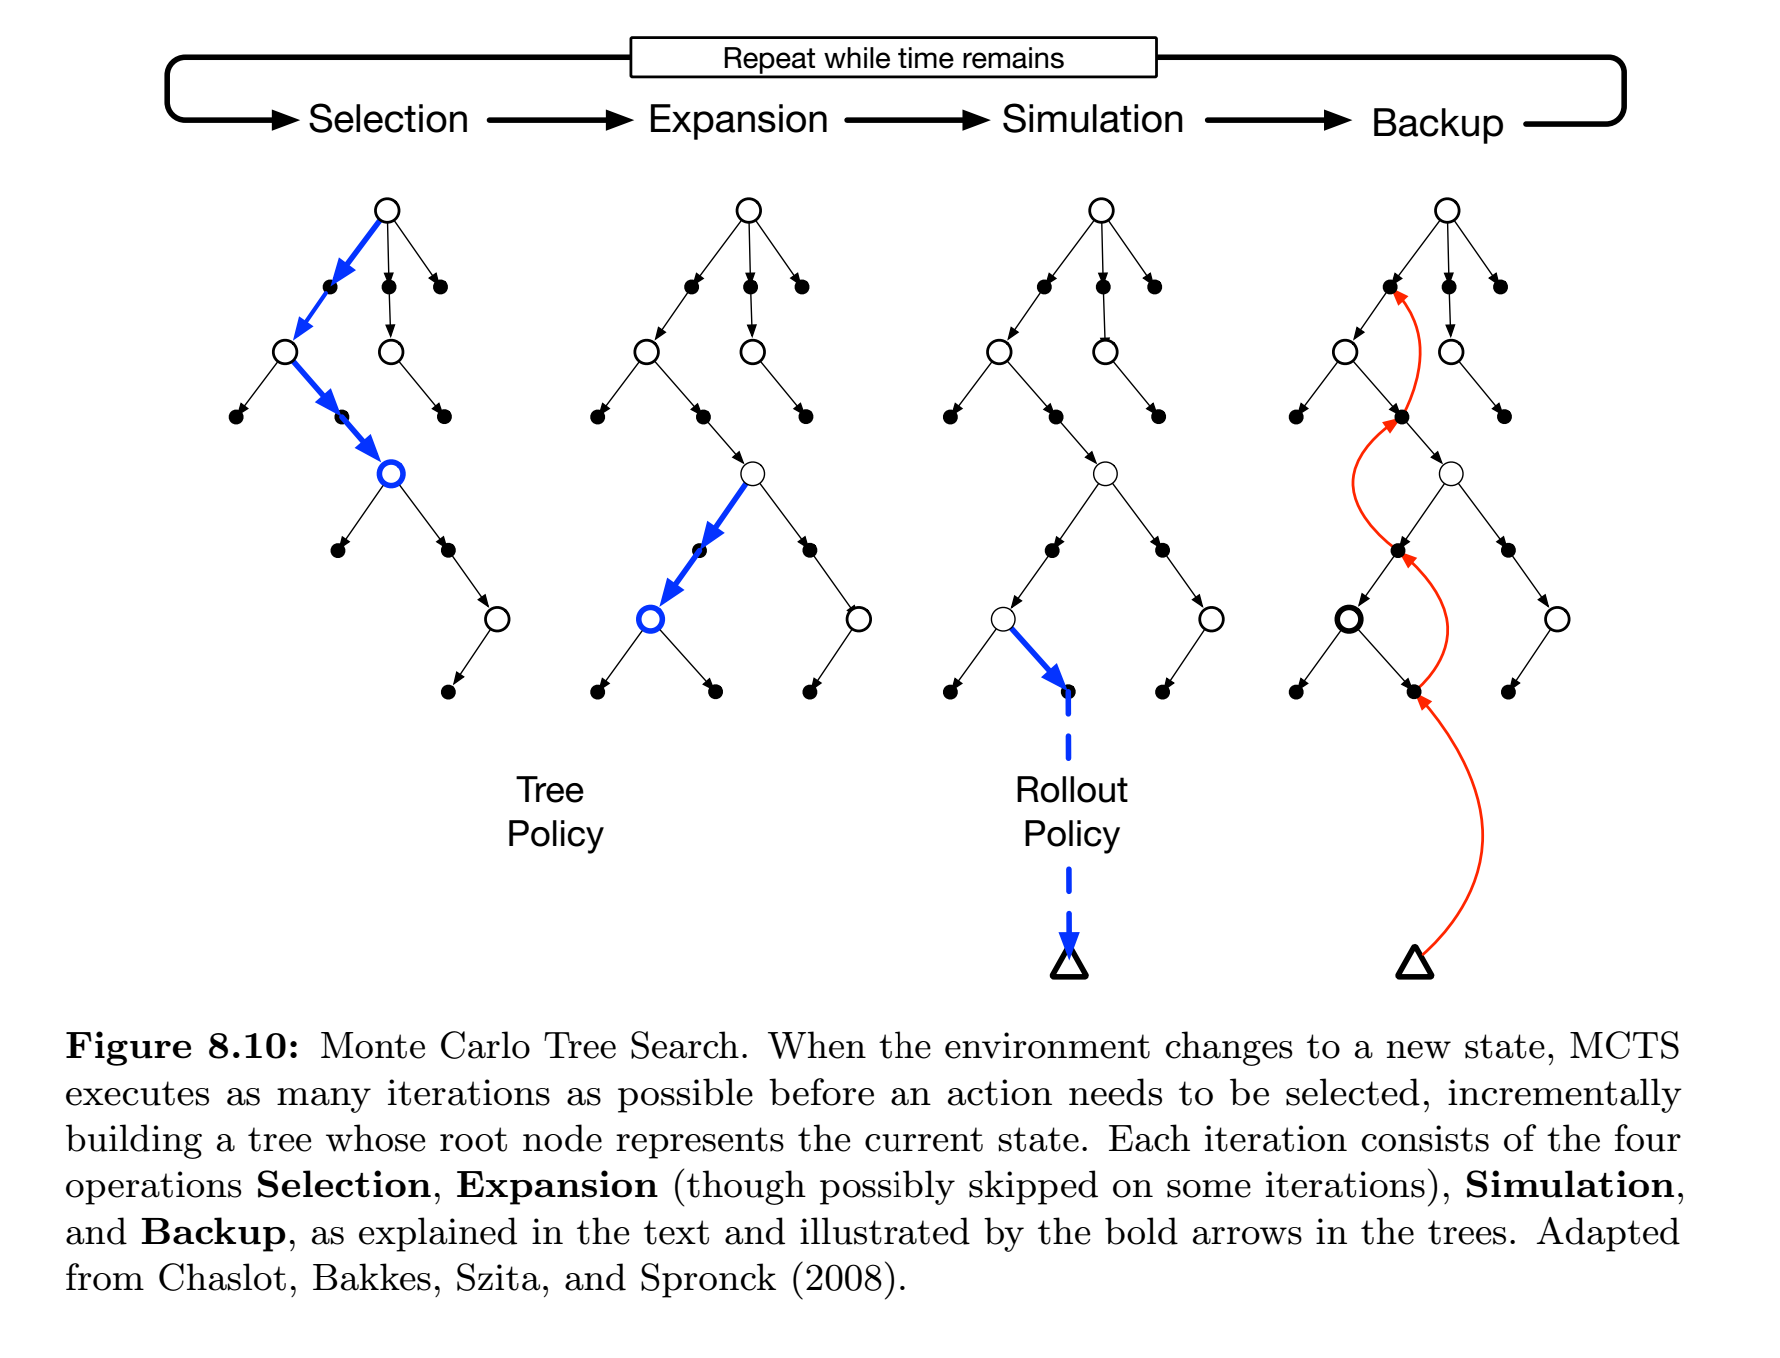
\includegraphics[width=450px,height=300px]{images/mcts}
    \caption{MCTS: Sutton Figure 8.10}
    \label{fig:my_label}
\end{figure}

The goal is to find the path through state space that will yield the highest return on average. You start with a game tree that only contains the root node. In the case of Go this would be the node representing the start of the game. You then proceed and repeat the following 4 steps as are represented in figure-1 for some predefined number of iterations. Once you have completed all iteration you will move on to the action phase in which you use the statistics built up in the tree to select an action in the actual environment. Each node in the tree associate with a unique state from the environment has the following statistics. For each possible action from the current state the state action value is represented by $Q(s,a)$. Visit count values for each state and action is represented by $N(s,a)$.

\begin{enumerate}
    \item \textbf{Selection}
    In this phase of the algorithm child nodes are selected until a leaf node is reached. Leaf node here means either a terminating node (game ending node) or a node that has not been explored yet. The child nodes are selected based on values of the edge connecting parent to child. This value can be assigned in different ways. An example is UCT (Upper confidence bound 1). The way exploration vs exploitation is balanced is using the following formula. 
    
    $ UCT = Q(s,a) + c*\frac{\sqrt{\sum{N(s,b)}}}{N(s,a) + 1} $
    
    includegraphics[width=300px,height=100px]{images/uct.png}
    
    \item Expansion
    
    Once a leaf node has been reached as long as its not a terminating node than add one or more child nodes of that leaf node to the tree. 
    \item Simulation
    
    From the selected child node run a simulation to the end of the episode (game). The simulation decisions use a rollout policy (off policy. Sometime uniform random) to select actions. This is usually done multiple times. So from the current selected node you would just select random actions until the game ends and save the result. You would repeat the process some number of times and then the average of those rollouts would be used as the estimate for the new node. 
    
    \item Backup
    
    The reward returned from the simulation is backed up through the edges of the tree that were used during the current episode. The reward is not saved to states that exist beyond the current tree. If the simulation step is run more than once then the average from the simulation step is backed up through the tree. If you are running MCTS for a two player game than you would flip the value of the return for the opponent node. If the node is a player one node for instance than all  player 2 nodes would get the negative of whatever player 1 received from the simulation outcome. If that was confusing we will see some examples that will help clarify. 
    
\end{enumerate}

As stated before these 4 steps would continue for a predefined number of iterations and then the acting step would commence. Remember those for steps were a \say{thinking} phase where from the current state the algorithm is thinking about what to do. Once the thinking phase is over the agent acts by selecting an action based off statistic in the tree. One common one is to select the action with the most visit counts or the action with highest value. 

Monte Carlo tree search is a decision time planning algorithm. A decision time planning algorithm is one in which a full simulation of planning is run on every state to produce each action. This is in contrast to \textit{background planning}. In background planning a policy or value function is gradually learned by simulated experience. The learning might happen at different time intervals. In short the two differences are this, decision time planning uses simulated experience to select an action in the current state whereas background planning uses simulated experience to improve a policy or value function and then uses that improved policy or value function to then select an action. 

For me this definition was a bit confusing and I suppose that there is likely some overlap in the two approaches in different algorithms. MCTS is a decision time algorithm because from the current state $S_t$ you might run the above 4 step 1k times or 10k times to accumulate statistics in the tree. Then once those simulations are over you will select an action from $S_t$ using the statistics accumulated in the tree. The mechanism for selection can be different from algorithm to algorithm. You might just select an action by trying to maximize value or you might take into account the number of times an action has been taken from $S_t$ in the past.

MCTS is also considered a rollout algorithm. \say{Rollout algorithms are decision-time planning algorithms based on Monte Carlo control applied to simulated trajectories that all begin at the current environment state. They estimate action values for a given policy by averaging the returns of many simulated trajectories that start with each possible action and then follow the given policy}.
(Sutton Page 152). 

(Leaving this out)
I list a few interesting properties that make MCTS a desirable algorithm.
\begin{enumerate}
    \item Planning time is independent of the size of the state space
    \item Need lots of samples to get a good estimate
    \item Running time is exponential in the horizon size. $O(|A|*n)^{H}$ where $A$ is the actions space. $n$ is the number of samples you want to run per simulation. $H$ is the horizon size
\end{enumerate}

\subsection{Example 1}

We will go through a quick toy example to understand each of the steps in MCTS. 
Below is a tree representing some game between two players blue and red. The current node of interest is the root node with value $ 5 / 10 $ (value / count) . 

We start in the select phase and the node has three actions (children nodes) to choose from. Using the UCT algorithm given above the algorithm would ascribe the following values to each node. Starting from the left most node and working right. Let $ c = 1 $

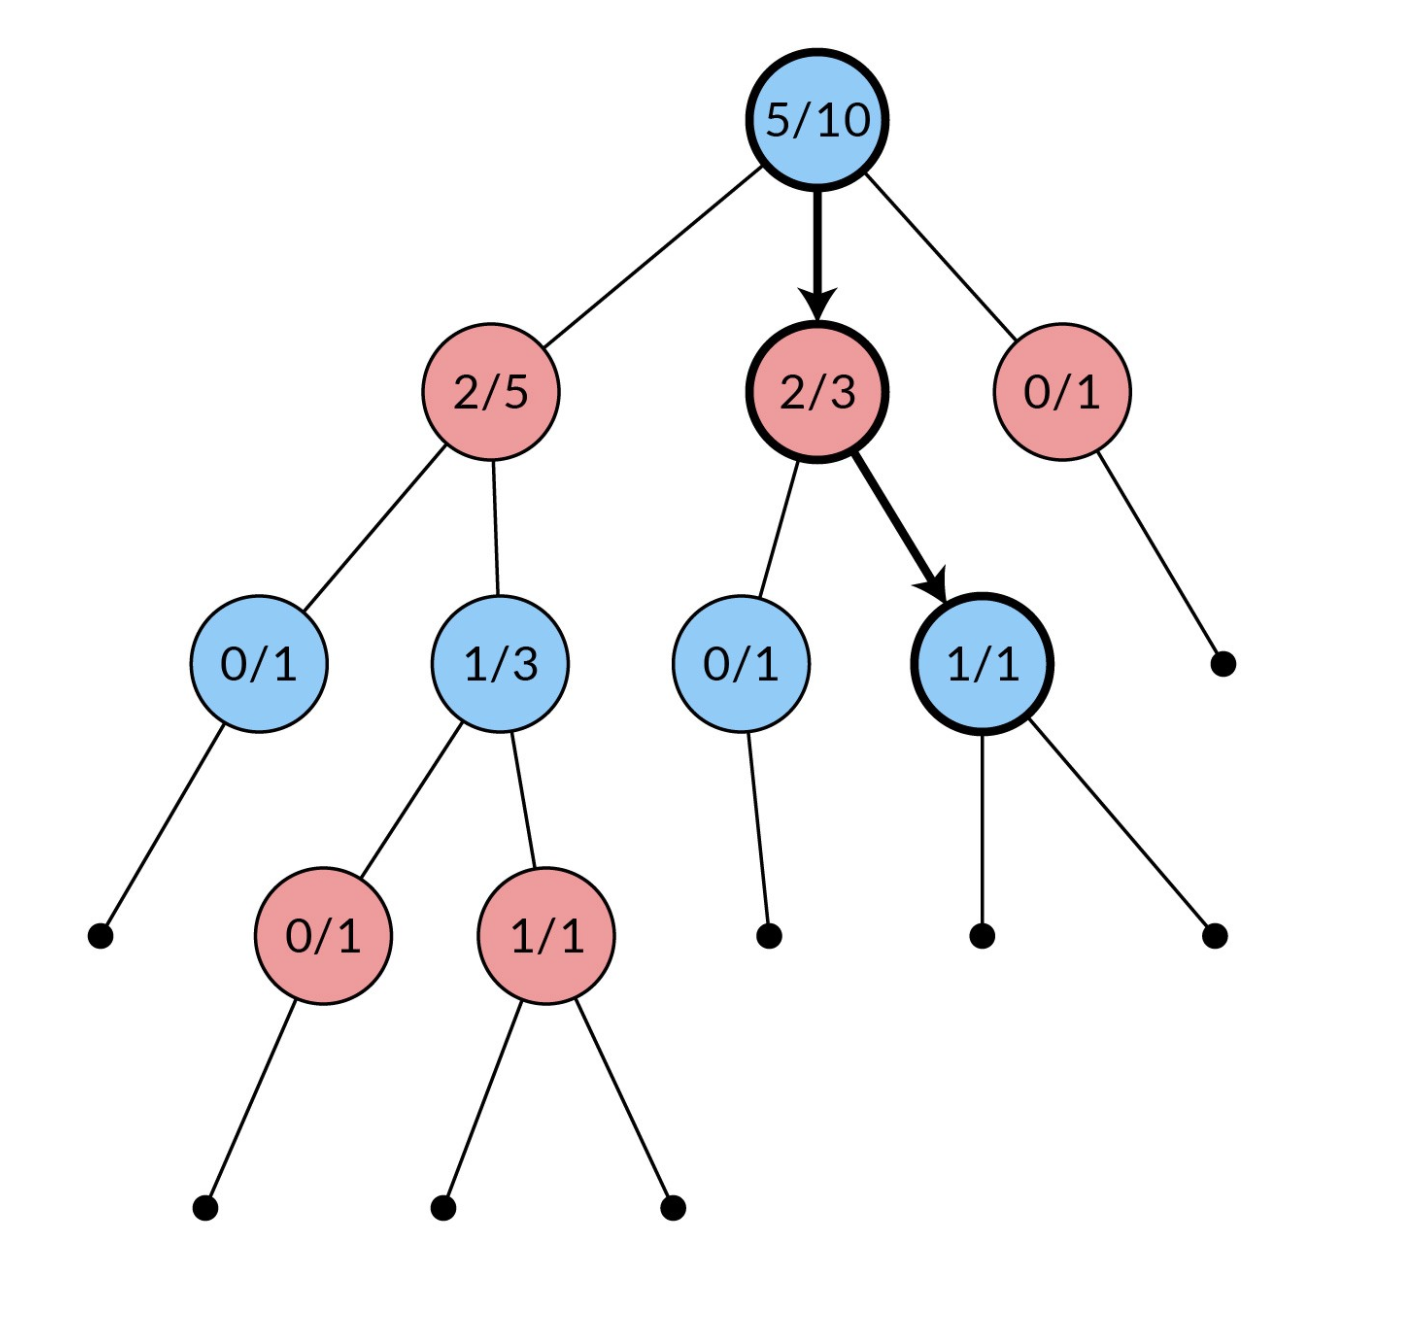
\includegraphics[width=200px,height=200px]{images/mcts_selection.png}

UCT(node1) = $ \frac{2}{5} + c \sqrt{\frac{ln({10})}{2}} = 1.07$

UCT(node2) = $ \frac{2}{3} + c \sqrt{\frac{ln({10})}{3}} = 1.54$

UCT(node3) = $ \frac{0}{1} + c \sqrt{\frac{ln({10})}{1}} = 1.51$

So we select node2 as is indicated with the bold arrow. Now for the children of node2 (node4,node5)

UCT(node4) = $ \frac{0}{1} + c \sqrt{\frac{ln({3})}{1}} = 1.048$

UCT(node5) = $ \frac{1}{1} + c \sqrt{\frac{ln({3})}{1}} = 2.048$

So we select node5 and since node5 is a leaf node we go to our expansion step.

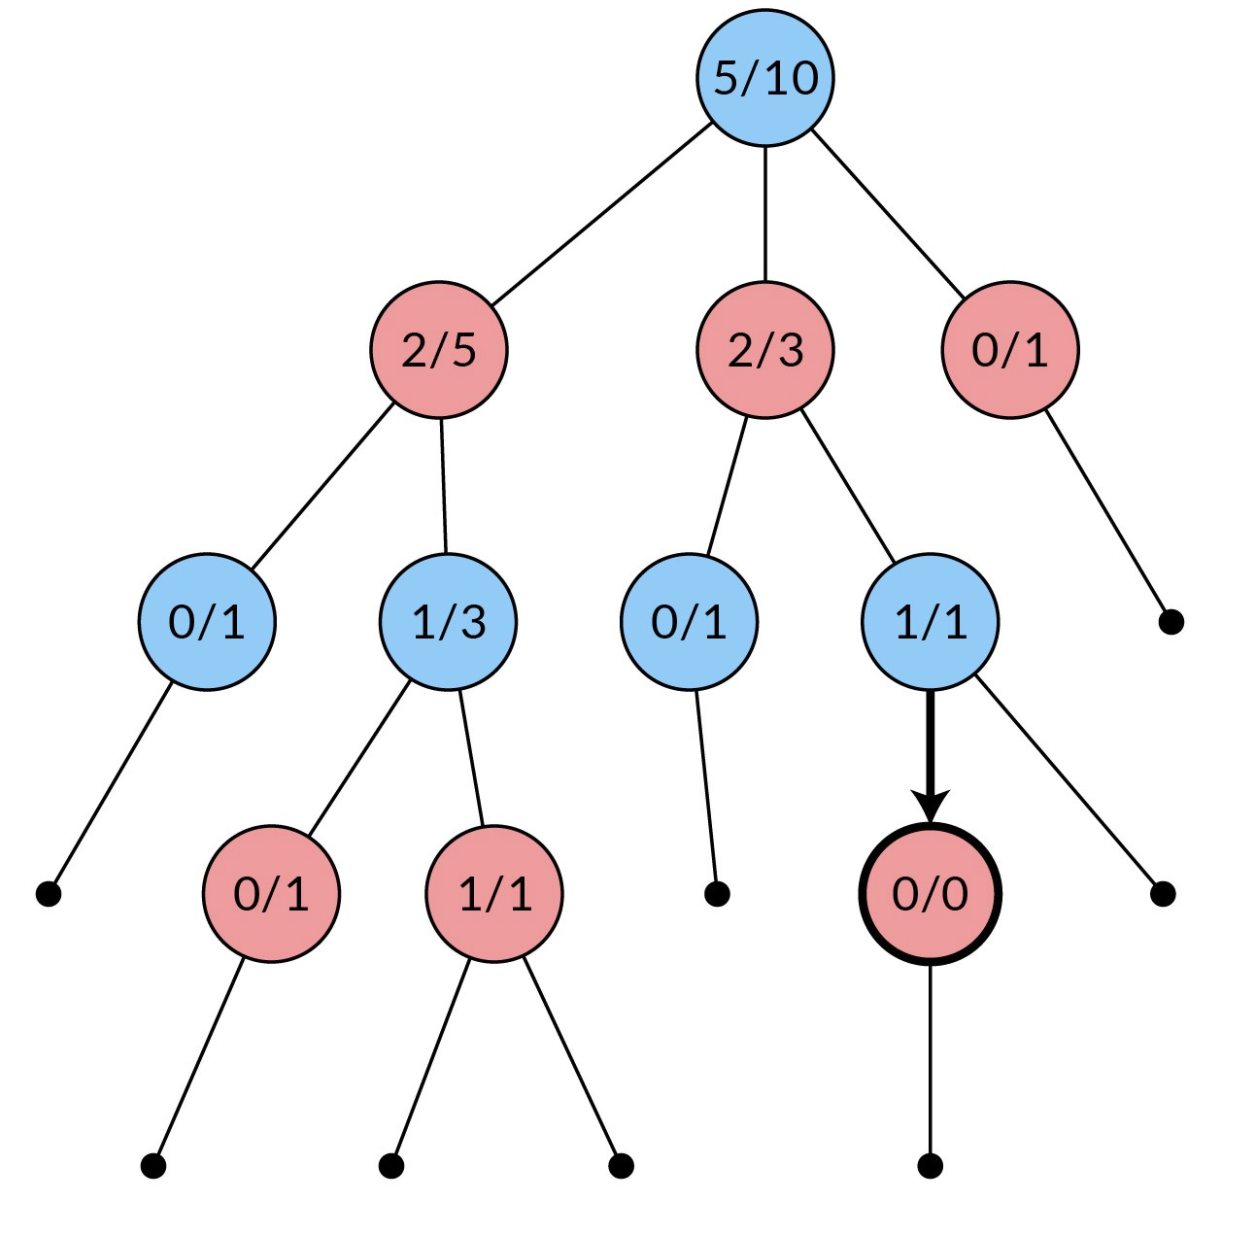
\includegraphics[width=200px,height=200px]{images/mcts_expansion.png}

We randomly select one of the two child nodes and assign the new node values of 0 / 0 (value / count). Now to estimate the value of the new node we run a rollout policy. This is usually random and so the agent will select random actions until a terminal node is reached. 

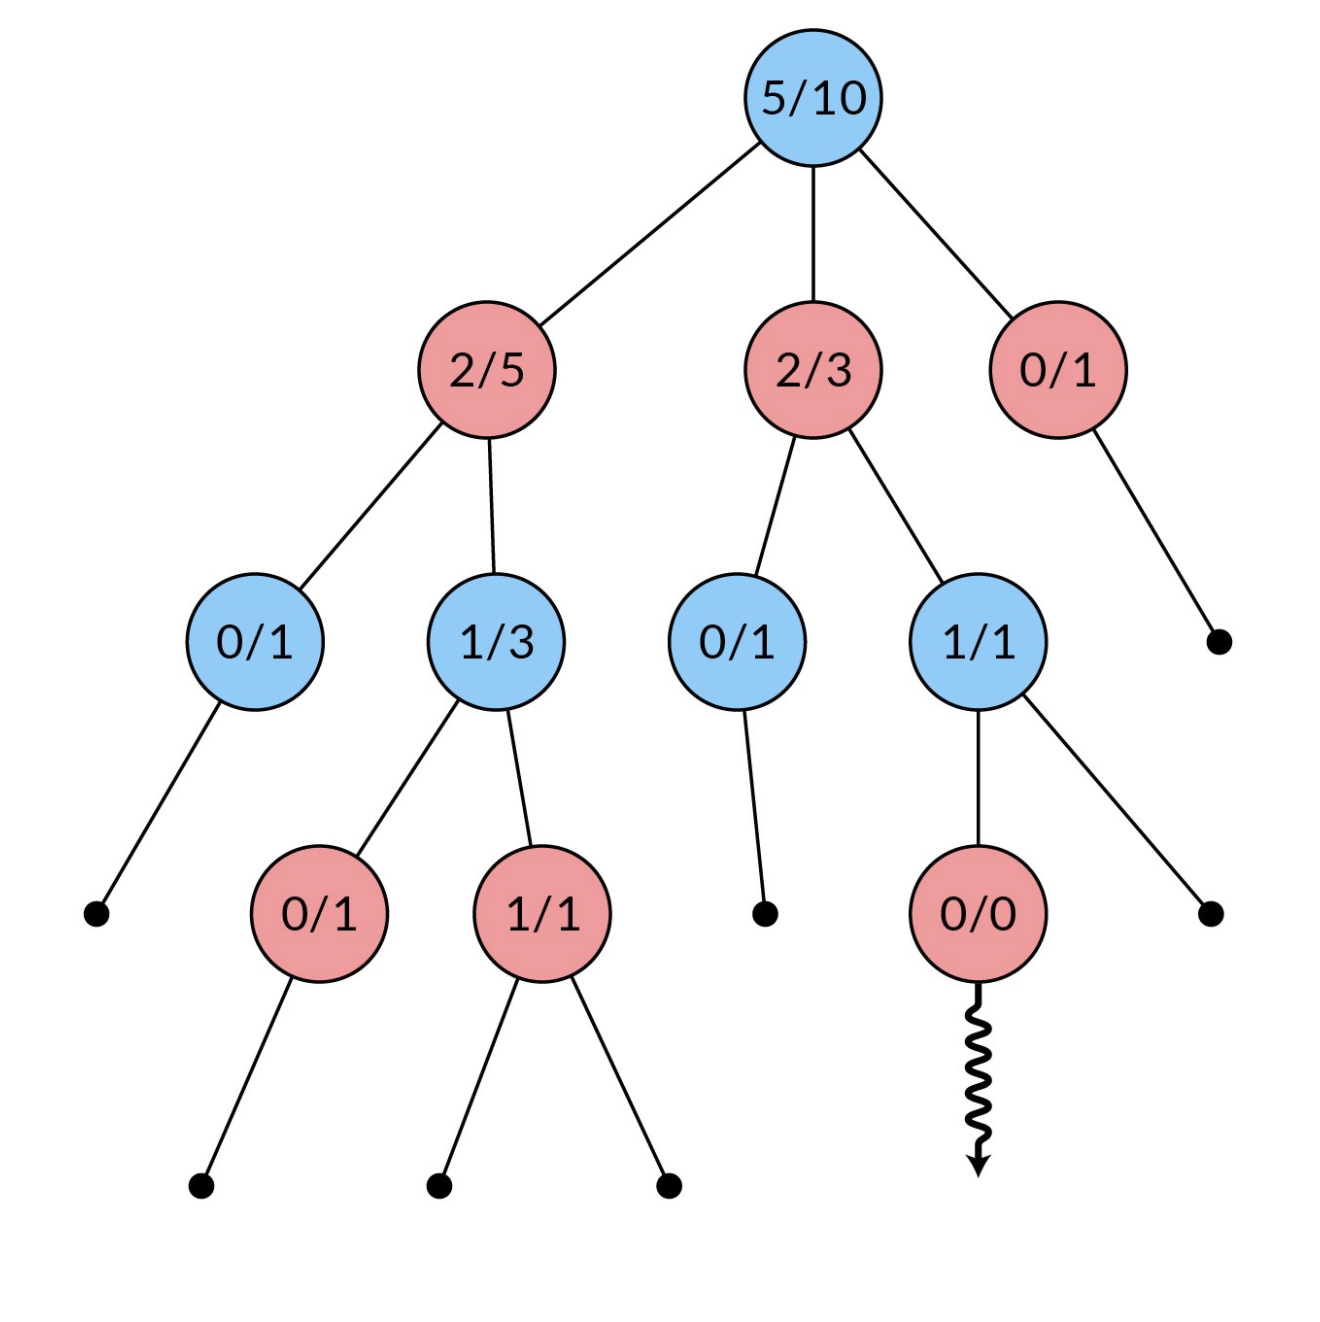
\includegraphics[width=200px,height=200px]{images/mcts_simulation.png}

In this example the terminal node was a win for blue and so now we can back up the values of the tree with this new result. Somewhat counter intuitively since blue wins that means we increase the value of all the red nodes along with their count but only increase the count values of all the blue nodes. This is because the red nodes are actions selected by blue and therefore since blue won that child node is more valuable to blue in the future. This is unique to multi player MCTS and you would not have to worry about this in a non-adversarial or cooperative setting. 

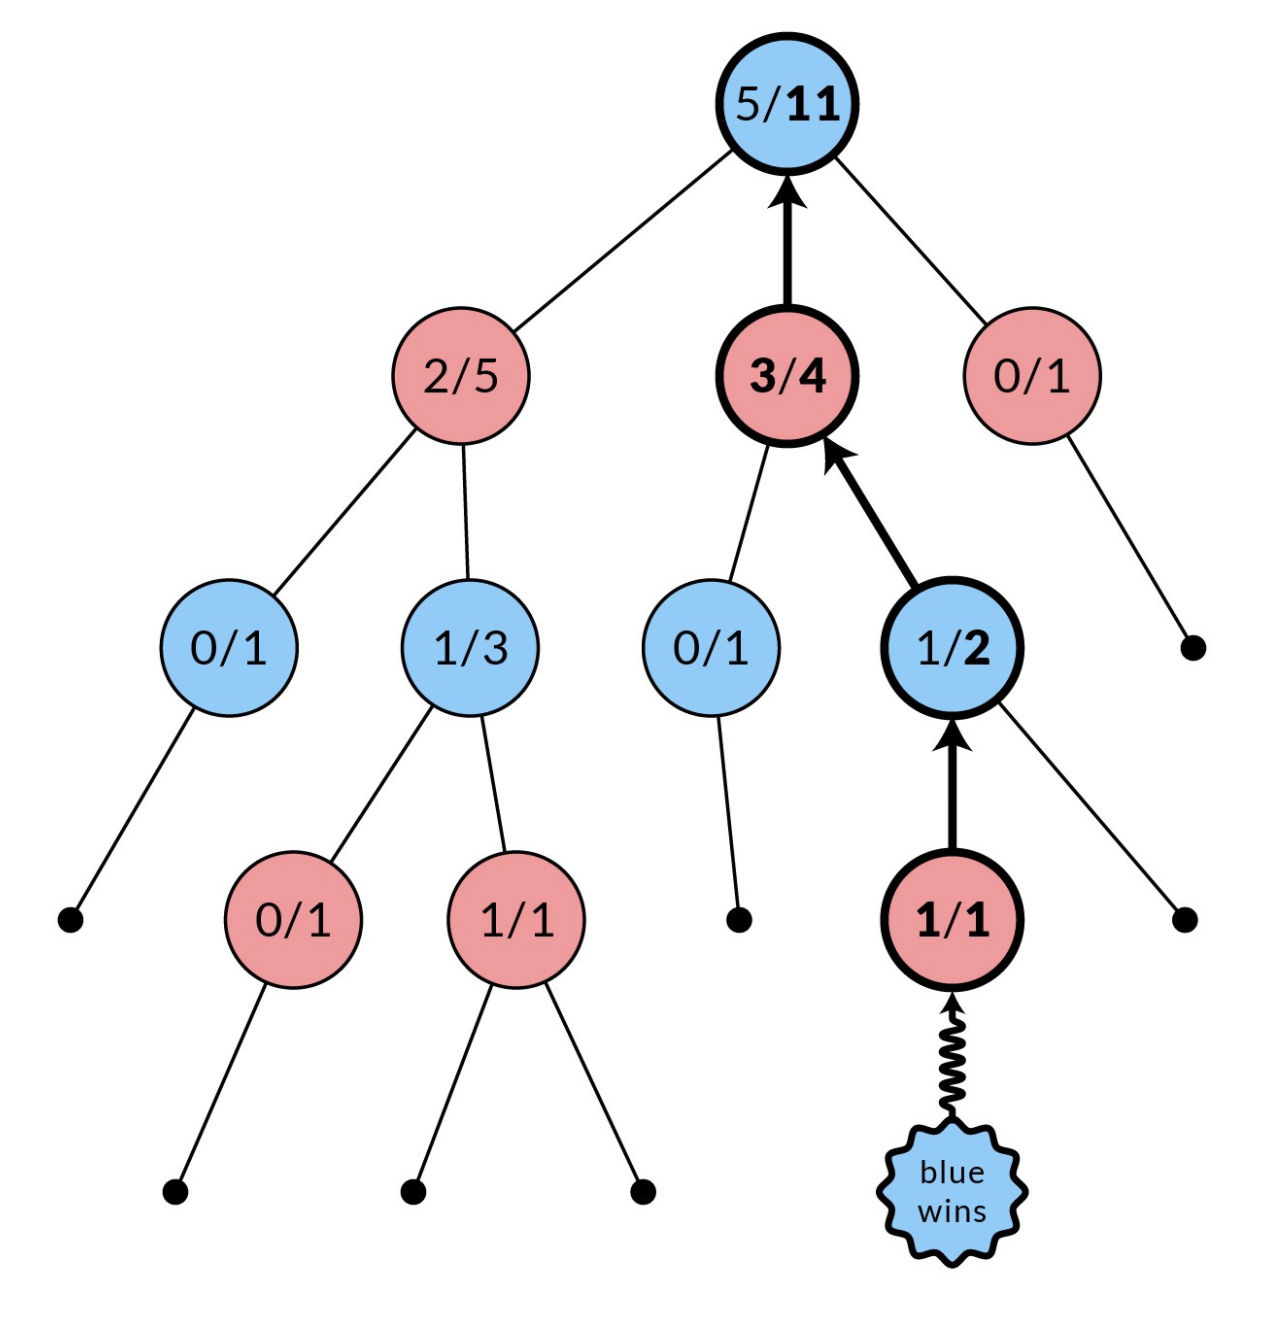
\includegraphics[width=200px,height=200px]{images/mcts_backpropagation.png}

\section{Multi Agent RL}

Let us now discuss how our previous discussed concepts in RL can be extended to the multi agent setting. Multi agent means that you have two or more players acting in the same environment with either opposing or aligned goals. We will stick to the zero-sum two player setting. Zero sum here means that the reward of one player comes at the expense of the other player. If one player wins the other must lose. Allowing for draws somewhat violates this if you allow for each player to receive some reward. In tictactoe we generally ascribe a reward of 0 for draws but there can be good reasons for at least giving an agent a small reward. 

Lets think back to the tictactoe example that we used to demonstrate the intractability of policy iteration for dynamic programming \ref{fig:tictactoe-dp}. Here we said that we needed $p(s^{'},r | s , a)$ in order to evaluate the current policy $\pi$. Well this probability in the context of a game like tictactoe is the probability of the other player taking a certain action from the state that you just presented to them. Previously we imagined that the environment just gave us this for free but certainly this is not the case in general. So how do we get the other players policy? There are a couple of possible approaches here. The first would be to try and estimate the other players policy from experience. You could for instance run some sort of rollout algorithm where you sample trajectories and maintain a lookup table of state-action observations for how often an opponent took an action given a state. So if out of 100 times of seeing state $s_{1}$ they take action $a_{1}$ 10 times then you would would describe their policy as $\pi_{p2}(a_{1}|s_{1}) = 0.10$. This approach would require maintaining a lookup table and so you would probably want to apply some function approximation technique to estimate a parameterized function for $\pi_{p2}$. This is a viable approach but it is not what was done in AlphaZero. AlphaZero uses a technique called self-play. 

\section{Self-Play}

Self-play is a concept that has been around in AI for a long time depending on how liberal your willing to be with the term AI. In 1951 Brown came out with a paper describing fictitious play a self-play algorithm In 1959 Checkers was solved using self-play with expert knowledge. There have been many other successes including AlphaZero. Self-play in short is any algorithm for which there are 2 or more players and the agent makes actions for every player. So the agent just plays against itself and improves play based off of what it observes during this self-play. This is easiest to see in zero sum two player games since they are symmetric. In this setting a self-play algorithm will play as both player 1 and player 2.The agent will play against itself switching perspectives between player 1 and player 2. AlphaZero does just this. We do this as humans occasionally when playing a game or perhpas other activities. For instance when thinking about how to develop better chess strategies you might see how well a strategy does by attempting to play against that strategy yourself and observing the outcome. 

This does not actually require learning two separate policies. It does however generally require adjusting how state is represented. We will add an encoding into the states representation to signify whose turn it is. This clearly designates one state from the other. In a game like tictactoe you can always see whos turn it is by simply looking how many pieces are on the board for each player. This is not true of other games like chess and Go however. So our policy will gives us a distribution over actions fro both the below state. The first for player "X" the other for player "O". 

\begin{figure}[H]
    \centering
    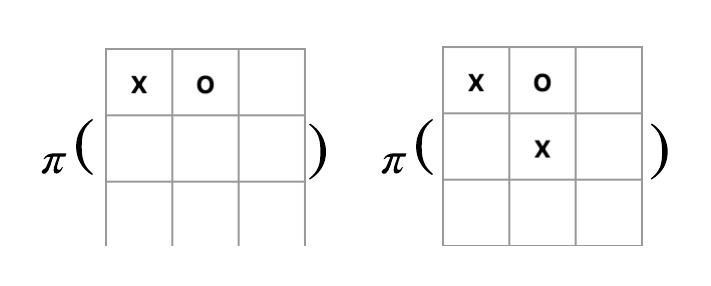
\includegraphics[width=200px,height=100px]{images/2playerpolicy.png}
    \caption{two player policy}
    \label{fig:2p-policy}
\end{figure}

\section{MiniMax and Alpha Beta Pruning}

The MiniMax algorithm is a classic game tree search algorithm. It can be used to arrive at guaranteed optimal solutions in two player zero sum games. 

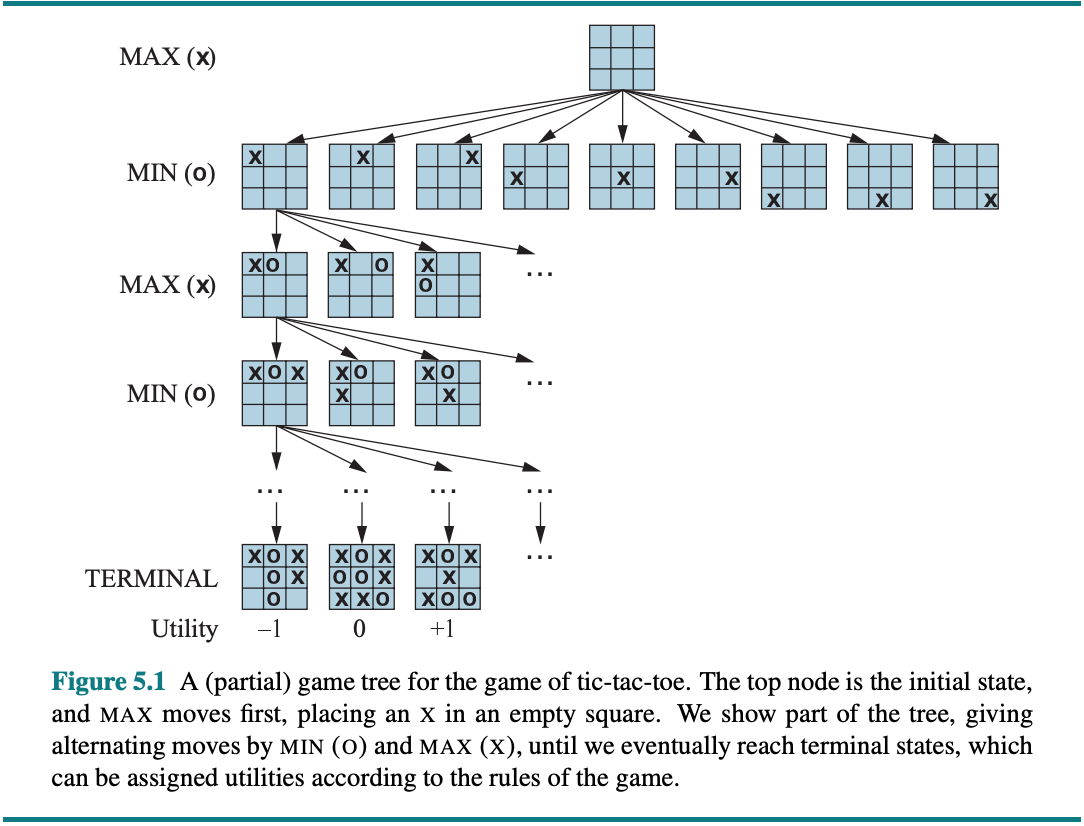
\includegraphics[width=350px,height=200px]{images/aim_figure_5_1.png}

Looking at figure 5.1 above taken from the classic text ``Artificial intelligence a modern approach" [2] we can view the game tree of a two player game as a game between a player MAX and a player MIN. It is player MAX's turn and he wants to maximize his utility. MIN knows that MAX is a greedy human and will be taking actions to maximize his own reward. What should MIN do? MIN will then take actions that will minimize the utility of MAX. MAX in turn knows about the devious plans of MIN and will take actions in accordance with this knowledge. That is to say that each player will act assuming that the other acts optimally. This setup gives rise to our first game-tree algorithm  
The optimal strategy of a given game tree can be determined by working out the minimax value of each state in the tree. The minimax value is the utility for the 
The MiniMax algorithm is the first game tree algorithm that we are going to look at. It is relevant for pedagogical purposes but we will also later use MiniMax as a baseline for comparison vs our more complex agents such as MCTS and AlphaGoZero. 

MiniMax Search Example: The example below demonstrates the algorithm with an oversimplified example. Moving left to right sarting with the max player. The leaf node values are already known. 

\begin{enumerate}
    \item Max player looks for max action over children nodes.  
    \item No value exists on the children nodes so MIN player finds the min action of the terminal states. First for the left node. Than the right. 
    \item MAX can now calculate the max of MIN's nodes. So in this toy example it is concluded that MAX should take the right action. 
\end{enumerate}

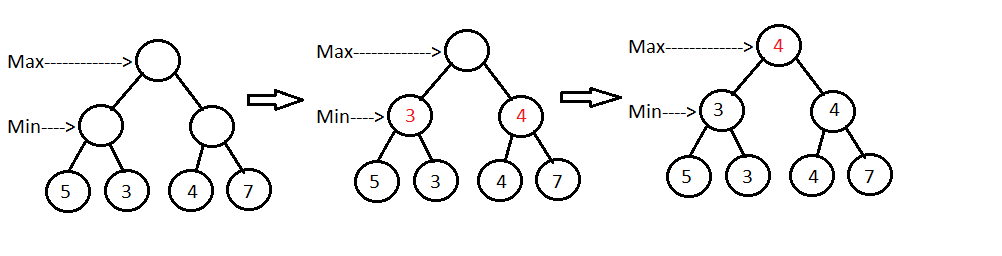
\includegraphics[width=300px,height=100px]{images/minimax_example.png}

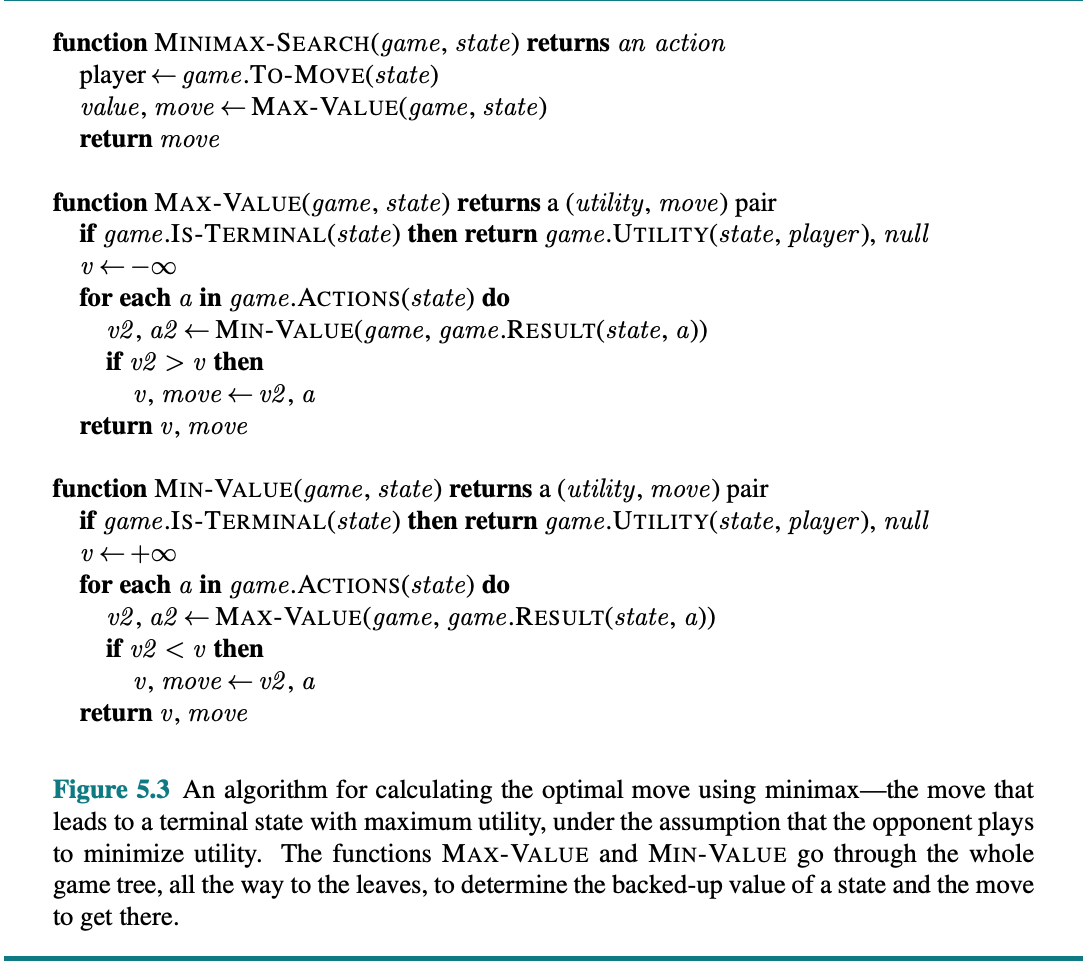
\includegraphics[width=300px,height=200px]{images/minimax_algo.png}

The pseudocode for the algorithm above can be implemented almost completely with three functions and a tree representation of whatever space your interested in. This algorithm is guaranteed to give you the optimal solution but is quite computationally expensive as every node needs to be visited at least once. One way to help reduce the search space is with alpha-beta pruning. The basic Idea of the algorithm is that there are points during the minimax search that searching further down a particular path is unnecessary to reach the optimal minimax decision. 

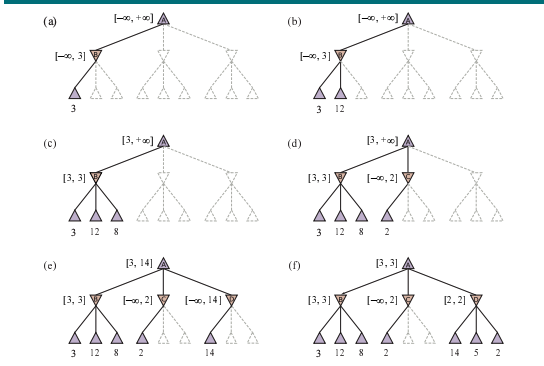
\includegraphics[width=300px,height=200px]{images/alpha_beta_figure.png}

The above figure [2] (fig 5.5) gives a nice example of why you dont need to search the entire tree. Let the two unsearched children nodes of node C be x and y respectively. Then the Minimax evaluation of the root node of the tree following the steps we just learning is evaluated like the following 

$ MINIMAX(s_{0}) = max(min(3,12,8), min(2,x,y), min(14,5,2)) $

$ = max(3,min(2,x,y),2) = 3 $ since $ min(2,x,y)$ will never evaluate to anything larger than 2 and 2 is less than 3 then the max player will never select node C and it is unecessary to know what x and y actually evaluate to. The figure below demonstrates this idea nicely. Consider the node n, if another node at the same level as n say $ m^{'}$ or another node further up the tree $m$ is better than n than we dont need to continue to explore n further. So as soon as we have enough information about $n$ to make this conclusion we can stop and prune whatever is left of $n$. Alpha-beta search as the name implies uses to values to help us know when pruning can take place.

\textbf{Alpha} - The value of the best choice we have found so far at any choice point along the path for MAX. 

\textbf{Beta} - The value of the best choice we have found so far at any choice point along the path for MIN. 

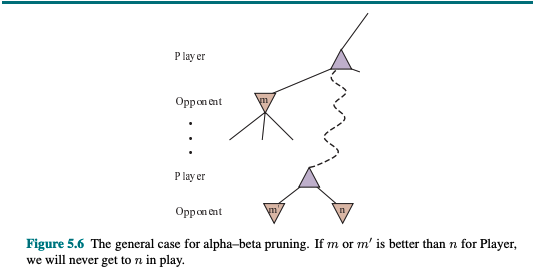
\includegraphics[width=400px,height=200px]{images/AI_figure_5_6.png}

Another nice way to represent this constraint is with the following graphic. Any node we are considering must be able to be between alpha and beta as represented by the number line. $ \alpha \leq N \leq \beta $


\includegraphics[width=400px,height=100px]{images/alpha_beta_number_line.png}



